%%%%%%%%%%%%%%%%%%%%%%%%%%%%%%%%%%%%%%%%%%%%%%%%%%%%%%%%%%%%%%%%%%%%%%
% How to use writeLaTeX: 
%
% You edit the source code here on the left, and the preview on the
% right shows you the result within a few seconds.
%
% Bookmark this page and share the URL with your co-authors. They can
% edit at the same time!
%
% You can upload figures, bibliographies, custom classes and
% styles using the files menu.
%
%%%%%%%%%%%%%%%%%%%%%%%%%%%%%%%%%%%%%%%%%%%%%%%%%%%%%%%%%%%%%%%%%%%%%%

\documentclass[12pt]{article}

\usepackage{sbc-template}

\usepackage{graphicx,url}

\usepackage[authoryear, round]{natbib}
\usepackage[brazil]{babel}   
\usepackage[utf8]{inputenc}  
\usepackage{float} % Para usar [H]
\usepackage{placeins} % Para usar \FloatBarrier
\usepackage{tikz}
 
\sloppy

\title{Proteger para Prevenir: Avaliação de Ferramentas Antivirus contra o uso do \textit{Keylogger} em Segurança da Informação\\ }

\author{Uriel do C. Andrade\inst{1},\\
Daniel de Oliveira Capanema\inst{1}, \\
Rafael Henriques Noqueira Diniz\inst{1}}


\address{Instituto de Ciências Exatas e Informática\\
Pontifícia Universidade Católica de Minas Gerais (PUC-MG)\\
Caixa Postal 1.686 – 30535.901 – Belo Horizonte – MG – Brasil
\email{uandrade@sga.pucminas.br}
\email{danielcapanema@pucminas.br, 557643@sga.pucminas.br}
}


\begin{document}

\maketitle
\begin{abstract}
    This paper presents an analysis of the effectiveness of tools for detecting and mitigating \textit{keyloggers}, focusing on solutions 
    that are widely used and accessible to end users. The study included tests on different formats of malicious files 
    (\texttt{.exe}, \texttt{.zip}, \texttt{.xlsm}), assessing the ability of these tools to detect and block threats. Antivirus programs such as Windows 
    Defender, Avast, AVG, Bitdefender, MalwareBytes, and Total AV were analyzed.
    The results revealed significant variations in the effectiveness of the tools depending on the format and approach used in the attack. The study identified which solutions performed better in the various tested scenarios, providing a detailed analysis of their capabilities and limitations.
    The conclusions contribute to the evaluation of the most effective solutions tested against \textit{keyloggers} in different attack contexts.
\end{abstract}
    

\begin{resumo}
    Este artigo apresenta uma análise da eficácia das ferramentas de detecção e mitigação de \textit{keyloggers}, com foco em soluções 
    amplamente utilizadas e acessíveis aos usuários finais. O estudo incluiu testes realizados em diferentes formatos de arquivos 
    maliciosos (\texttt{.exe}, \texttt{.zip}, \texttt{.xlsm}), avaliando a capacidade dessas ferramentas de detectar e bloquear 
    ameaças. Foram analisados antivírus como Windows Defender, Avast, AVG, Bitdefender, MalwareBytes e Total AV.  
    Os resultados evidenciaram variações significativas na eficácia das ferramentas, dependendo do formato e da abordagem empregada no ataque. O estudo identificou quais soluções apresentaram melhor desempenho nos diversos cenários testados, fornecendo uma análise detalhada de suas capacidades e limitações.  
    As conclusões contribuem para a avaliação das soluções mais eficazes testadas contra \textit{keyloggers} em diferentes contextos de ataques.
\end{resumo}
    
\section{Introdução}

Nos últimos anos, os avanços tecnológicos, como a popularização dos smartphones e a introdução da inteligência artificial, transformaram a sociedade, tornando-a mais conectada e digital. No entanto, com essas inovações, surgiram também desafios significativos para a segurança cibernética, especialmente com o aumento das ameaças digitais.

\textit{"Na era da Indústria 4.0 (IR 4.0), o vazamento de informações se
tornou um problema crítico para a segurança da informação."} \citep{bhaharin2019issues}

Os \textit{malwares}, como os \textit{keyloggers}, são um dos exemplos dessas ameaças. 
Esses programas maliciosos, que funcionam de forma furtiva, capturam pressionamentos de tecla,
expondo os usuários a riscos de roubo de informações diversas. \textit{"Os dados
capturados incluem senhas, IDs de usuários, conteúdo de documentos
e outras informações críticas; portanto, um invasor pode obter dados
confidenciais sem invadir o banco de dados ou arquivo."} \citep{ahmed2014survey}

Dada a constante evolução dessas ameaças, é fundamental implementar métodos de defesa cada vez mais eficazes para proteger a privacidade e a segurança dos usuários em um mundo digital em constante transformação.

\subsection{Problema}

%algum numero que reforce o problema. No mundo 3 bilhões são perdido por ataques. e colocar referência.

Apesar dos inúmeros benefícios proporcionados pelos avanços tecnológicos, os riscos aumentaram proporcionalmente quando o assunto envolve os dados de seus usuários e organizações neste ambiente digital.

\textit{Keyloggers} são uma ameaça crescente que afeta pessoas e organizações em todo o mundo, causando sérios danos e comprometendo informações importantes. Estima-se que as perdas com crimes cibernéticos chegarão a USD 10,3 bilhões em 2022, com foco em fraudes de e-mail comercial (BEC) e surtos de ransomware, impactando empresas e usuários finais. O phishing, frequentemente associado a \textit{keyloggers}, é o crime cibernético mais comum, com mais de 300 mil reclamações recebidas no mesmo ano \citep{securityintelligence2023}.

Dada a confidencialidade destes serviços e a sua capacidade de operar em muitas áreas, é importante desenvolver estratégias eficazes para reduzir estes riscos. É importante analisar e comparar métodos de combate aos \textit{keyloggers} para garantir que os benefícios desta ferramenta não sejam comprometidos pelos perigos que pode causar. Compreender os perigos destes riscos e implementar medidas de segurança fortes é crucial para proteger dados e informações importantes.

\subsection{Objetivo principal}
O objetivo principal deste trabalho é, por meio de um ambiente controlado 
investigar o funcionamento do \textit{keylogger} 
e realizar uma análise comparativa entre diferentes ferramentas de detecção e mitigação de vírus.

Esta análise será conduzida comparando 6 ferramentas de proteção, 
avaliando aspectos como: qual detecta o \textit{keylogger}, 
sua eficiência na detecção e as medidas tomadas após o \textit{keylogger} ser identificado. Dessa forma, 
o estudo pretende identificar as soluções mais completas e acessíveis, visando fortalecer 
as estratégias de segurança digital tanto para profissionais quanto para usuários comuns.

\subsection{Objetivos específicos}

Os objetivos específicos desta pesquisa são:
\begin{itemize}
    \item Criar um ambiente controlado para analisar os mecanismos de operação dos \textit{keyloggers}, observando como eles capturam dados.
    \item Avaliar a eficácia de antivirus presentes no mercado quanto a sua detecção e mitigação para os \textit{keyloggers}.
    \item Realizar uma análise comparativa entre as ferramentas de segurança, destacando quais são mais eficientes na prevenção de \textit{keyloggers} em diferentes cenários.
    \item Fornecer recomendações baseadas em resultados empíricos sobre os melhores softwares de proteção 
    na detecção e neutralização de \textit{keyloggers}, contribuindo para o aprimoramento da segurança digital.
\end{itemize}

\subsection{Contribuições Esperadas}
A partir da elaboração do trabalho e obtenção dos resultados, espera-se que este estudo contribua para a comunidade técnica e científica ao oferecer uma análise detalhada da eficácia de métodos \textit{anti-keylogger}. Dado que as pesquisas sobre este tema, especificamente em sistemas operacionais de uso comum, são limitadas, este trabalho possibilitará a comparação entre diferentes ferramentas de detecção e mitigação de \textit{keyloggers}, oferecendo insights sobre as soluções mais eficientes para o problema em questão.

\section{Fundamentação teórica}

\subsection{Segurança da informação}
A segurança da informação é uma preocupação crítica para organizações no cenário digital contemporâneo. Como destaca \citep{bhaharin2019issues} , a proteção e segurança das informações organizacionais têm se tornado cada vez mais desafiadoras na era da Indústria 4.0. Isso é atribuído ao surgimento de ameaças sofisticadas à segurança.

O surgimento da Indústria 4.0 trouxe conectividade sem precedentes e integração de tecnologias digitais nos processos organizacionais. Embora essa conectividade tenha facilitado a eficiência e a inovação, também expôs as organizações e seus usuários a uma ampla gama de ameaças cibernéticas. Desde software malicioso e ataques de \textit{phishing} até violações de dados e ameaças internas, o cenário de ameaças moderno é caracterizado por sua complexidade e diversidade.
\subsection{\textit{Malware}}
\textit{Malwares}, abreviação de malicious software (software malicioso), são definidos como códigos ou programas desenvolvidos com a intenção de causar danos a sistemas, roubar informações ou prejudicar seu funcionamento sem o consentimento do usuário. Representam uma ameaça crescente e complexa no mundo digital, sendo disseminados por diversos meios, como e-mails, sites ou dispositivos infectados \citep{singh2021keylogger}.

Neste mesmo contexto, é relatado pelo \citep{singh2018infringement} que \textit{"aproximadamente 1 milhão de arquivos de \textit{malware} são criados todos os dias, e o crime cibernético prejudica a economia mundial em aproximadamente USD 6 trilhões anualmente, até 2021"}.
\subsection{\textit{Keylogger}}
De acordo com \citep{wajahat2019novel}, \textit{"\textit{keyloggers} são ferramentas de monitoramento que possui uma certa ou total capacidade de capturar cada pressionamento de tecla de um teclado e armazenar em arquivos de log."}

Também conhecidos como registrador de pressionamentos de tecla, os \textit{keyloggers} é um tipo de \textit{spyware}, que podem ser utilizados tanto em contextos éticos quanto em situações que desconsideram a ética. Em contextos éticos, eles são empregados em empresas onde \textit{"o monitoramento é um fator importante para manter a estabilidade da rede"} \citep{tuli2013system} e para realizar a vigilância de crianças na navegação à internet. No entanto, em cenários onde a ética não é levada em conta, \textit{keyloggers} podem ser usados de forma maliciosa para roubo de informações pessoais, como senhas e dados bancários, espionagem ou outras atividades ilícitas.

Existem dois tipos principais de variações dessa ferramenta, cada uma com suas peculiaridades e mecanismos de funcionamento distintos. O primeiro tipo é o \textit{keylogger} de hardware, \textit{}\citep{singh2021keylogger}. Após os dados serem salvos na memória interna eles podem ser acessados de várias maneiras, dependendo do design do dispositivo e das intenções do atacante.

O segundo tipo é o de software, um programa que é instalado no sistema do computador. \textit{O keylogger de software intercepta dados que viajam pelo teclado e pelo sistema operacional. Ele coleta eventos de pressionamento de tecla, armazenando-as em um local remoto e depois os transmite ao invasor que instalou o keylogger} \citep{ahmed2014survey}.

\subsection{Heuristicas de detecção}
Heurísticas de detecção são técnicas avançadas usadas para identificar ameaças que não são detectadas por métodos tradicionais. Algumas das principais são:

Técnica de anti-hook: Esta tecnologia é baseada no uso de ganchos de API, que são utilizados por todos os processos (visíveis ou ocultos) para implementar ganchos. Hooks são um conjunto de métodos usados para alterar o comportamento de um sistema operacional ou aplicativo. Isto pode interromper o fluxo de chamadas de função ou mensagens entre diferentes componentes do computador. O sistema verifica todos os processos, executáveis estáticos e DLLs (bibliotecas de vínculo dinâmico) para identificar processos ou arquivos suspeitos que usam ganchos \citep{solairaj2016keyloggers}.

Técnica HoneyID: \citep{10124477} \textit{"É ferramenta capaz de atrair e capturar o invasor, servindo para enganar e monitorar suas atividades"}. Ele opera como um honeypot, criando iscas no sistema para atrair invasores, registrando suas interações suspeitas e coletando informações sobre seus comportamentos.

Detecção Baseada em Assinaturas: É uma técnica usada por antivirus para identificar malware com base em padrões específicos já conhecidos. É eficaz para detectar ameaças registradas, mas não consegue identificar malware novo ou desconhecido \citep{aslan2020comprehensive}.

\section{Trabalhos relacionados}

A análise sobre a ação dos \textit{keyloggers} fornece uma visão detalhada sobre a definição, os diferentes tipos e as técnicas de detecção e prevenção, conforme discutido por \citep{singh2021keylogger}. O autor aborda amplamente a importância de proteger informações confidenciais contra esses programas maliciosos e apresenta métodos proativos, como o uso de softwares \textit{anti-malware} e a verificação de entradas de inicialização. O trabalho também destaca estratégias específicas para dispositivos móveis, considerando suas características distintas.

Focando em \textit{keyloggers} de software, \citep{wajahat2019novel} aprofundaram a análise de suas operações tanto em modo kernel quanto no espaço do usuário, ilustrando exemplos históricos de uso malicioso, como o roubo de credenciais bancárias. Esses autores propuseram uma solução baseada na simulação de teclas e padrões de entrada/saída, demonstrando eficácia na detecção e aplicabilidade prática, especialmente em dispositivos móveis.

Para \citep{solairaj2016keyloggers} uma ampla gama de técnicas de detecção, incluindo abordagens baseadas em assinaturas e comportamentos, como Anti-Hook e HoneyID. Além disso, propuseram o uso de Support Vector Machines (SVM) para aprimorar a detecção de \textit{keyloggers}. Essa técnica, particularmente relevante para dispositivos móveis, mostrou-se eficaz na superação de desafios específicos, proporcionando maior precisão na identificação de ameaças. Por outro lado, \citep{aslan2020comprehensive} voltaram-se para métodos avançados de detecção de \textit{malware}, como o aprendizado profundo, aplicando-os ao combate de \textit{keyloggers}. A pesquisa evidenciou o potencial dessas técnicas para identificar padrões complexos e oferecer soluções robustas e adaptáveis a diferentes plataformas, com especial foco em dispositivos móveis.

Avanços significativos têm sido feitos na detecção e 
bloqueio de \textit{keyloggers} nos últimos anos. Estudos como os de \citep{singh2021keylogger}, 
\citep{wajahat2019novel}, \citep{solairaj2016keyloggers} e \citep{aslan2020comprehensive} destacam técnicas 
inovadoras na área. Este trabalho, porém, avalia ferramentas que aplicam essas técnicas, 
priorizando sua acessibilidade e eficácia em cenários reais.

Os artigos mencionados forneceram conceitos fundamentais que embasaram este estudo, 
auxiliando no desenvolvimento do trabalho.
\section{Metodologia}
\subsection{Ambiente}
Um passo crucial para garantir o sucesso do monitoramento, adaptação e codificação é a seleção cuidadosa das ferramentas adequadas para segurança e implementação.

Compondo o ambiente de teste como sistema operacional base, 
o Ubuntu (24.04) foi escolhido, principalmente devido à familiaridade com o SO, 
o que facilita a execução dos testes e a resolução de possíveis problemas. 
Além disso, a escolha também se deu pelo fato do Ubuntu ser uma distribuição Linux, 
pressupondo que este é um sistema operacional seguro no que diz respeito a invasão e contaminação de dispositivos.

Para garantir um isolamento adicional e mais segurança, 
a ferramenta de virtualização (um programa que cria ambientes isolados dentro do computador
para testes ou execução de diferentes sistemas sem afetar o sistema principal) VirtualBox (7.1.2) foi instalado sob o Ubuntu.
Ambas as ferramentas foram selecionadas não só pela segurança que proporcionam, 
mas também pela maior afinidade com elas.

Como Sistema operacional virtualizado, o Windows 10 foi escolhido para os testes devido à sua ampla utilização global,
com mais de 60\% de participação no mercado, o que o 
torna um alvo comum para \textit{keyloggers} e malware \citep{tomshardware2023}. 
Essa popularidade não apenas torna os testes mais relevantes, mas também
permite avaliar a eficácia das ferramentas de detecção em um ambiente 
amplamente explorado por atacantes e amplamente utilizado por usuários, 
refletindo cenários próximos à realidade.

\subsection{Seleção do \textit{keylogger}}
Para esta parte do projeto, envolve uma busca e seleção de um código de \textit{keylogger} já existente, que será utilizado como base para a realização dos testes e validações necessárias. O objetivo é encontrar um código que implemente as funcionalidades básicas de um \textit{keylogger}, permitindo assim concentrar esforços nas etapas de testes, depuração e validação, sem a necessidade de desenvolvimento inicial do código. Uma vez identificado o código, as etapas do processo incluem:

\begin{itemize}
    \item \textbf{Análise do Código}: Será realizada uma análise detalhada do código escolhido, buscando entender sua estrutura, funcionalidades e fluxo de execução.
    \item \textbf{Teste e Depuração}: Para esta etapa, 
    foi utilizado o Visual Studio Code (1.94), desenvolvido pela Microsoft. 
    A escolha se deve à familiaridade com a ferramenta e à afinidade com os recursos que seu ambiente 
    proporciona. Por ser um editor de texto leve e extensível 
    (ou seja, ele é capaz de ser personalizado com extensões para adicionar  
    funcionalidades como suporte a linguagens de programação e o IntelliCode), 
    o VS Code foi fundamental para facilitar os processos de teste e depuração do código do \textit{keylogger}.
    \item \textbf{Implementação de Funcionalidades}: Caso necessário, novas funcionalidades poderão ser implementadas, como a otimização do envio de dados e a melhoria da captura de informações.
    \item \textbf{Build e Distribuição}: Após a validação do código, será realizada a compilação utilizando o \textit{PyInstaller} para gerar um arquivo executável (.exe) que poderá ser utilizado em sistemas Windows.
    \item \textbf{Teste de Eficiência}: Será realizado um teste de eficiência para verificar o desempenho do \textit{keylogger} e sua capacidade de evadir detecção por antivirus.
\end{itemize}

\subsection{Seleção das ferramentas de antivirus para teste}
Nesta pesquisa, serão avaliados métodos para interceptar \textit{keyloggers}, 
com a instalação de ferramentas \textit{anti-malware}. 
A seleção das ferramentas será baseada nas mais utilizadas no mercado, 
acessíveis ao público geral e intuitivas. Esse critério visa garantir um teste que apresente
soluções, que sejam úteis tanto para usuários leigos, quanto para profissionais.

\subsection{Teste das Ferramentas de segurança para Detectar Keyloggers}
Durante esse processo de teste, os resultados serão obtidos por meio da aplicação 
da metodologia \textit{Real World Prevention Test} (RWPT), que avalia como as soluções 
de segurança se comportam em condições que refletem ameaças reais, ou seja, em 
situações mais próximas daquelas enfrentadas pelos usuários no cotidiano. 

Essa abordagem permite examinar, 
de forma contextualizada, o desempenho das soluções, 
oferecendo uma avaliação mais precisa de sua eficácia em um cenário real. 
O critério de avaliação das ferramentas verificará qual delas detecta o \textit{keylogger}, 
sua eficiência na detecção e as medidas tomadas após o \textit{keylogger} ser identificado. 
Para cada método de infecção (.exe, .zip, .xlsm), serão realizados cinco testes por ferramenta, 
a fim de avaliar a consistência da detecção.
\section{Desenvolvimento}

\subsection{Configuração do Ambiente}

Durante esta fase, foi instalado o VirtualBox, escolhido para fornecer 
um ambiente controlado e seguro para os testes. Em seguida, foi instalada 
com sucesso uma imagem ISO do Windows 10 na máquina virtual (ISO é um arquivo 
que contém uma cópia exata do sistema operacional, funcionando como um "arquivo 
de instalação" que pode ser usado para configurar o sistema). 
A instalação foi concluída sem problemas, permitindo que o sistema operacional 
funcionasse adequadamente. Dessa forma, o ambiente foi preparado para rodar os testes.
\subsection{Sobre o código \textit{Keylogger}}

Na busca por um código de \textit{keylogger}, foi encontrado um que atendia aos padrões e objetivos do trabalho. Desenvolvido em Python e disponível no GitHub, o código, criado pelo autor \citep{Aydinnyunus}, foi submetido a um processo de testes, depuração e compilação para garantir sua eficácia e segurança. Este \textit{keylogger} pertence à categoria de \textit{keyloggers} de software, sendo capaz de monitorar entradas do teclado e capturar cliques do mouse. Projetado para roubar os dados coletados, o \textit{keylogger} envia automaticamente as informações por meio de e-mails.

\subsubsection{Funcionamento}

O código do \textit{keylogger} desenvolvido por \textit{Yunus} utiliza técnicas de multithreading, permitindo a execução simultânea de várias tarefas sem comprometer o desempenho do sistema. A captura de dados ocorre de maneira eficaz e em tempo real, sendo gerenciada por quatro \textit{threads} principais, cada uma com uma tarefa específica:

\begin{itemize}
    \item \textbf{Captura do Mouse}: Uma thread dedicada à captura dos movimentos e cliques do mouse, garantindo que todas as interações do usuário sejam monitoradas.
    \item \textbf{Captura do Teclado}: Responsável por registrar as teclas pressionadas, armazenando esses dados ou enviando-os posteriormente.
    \item \textbf{Thread Principal}: Controla a execução do programa e a sincronização entre as demais threads, assegurando que o \textit{keylogger} funcione corretamente.
    \item \textbf{Envio de Dados}: Responsável por enviar os dados capturados para o 'hacker'.
\end{itemize}

Para simular o envio de e-mails com os dados capturados, o \textit{keylogger} se integra com a API Mailtrap, uma ferramenta que simula a rede de e-mails e permite testar a funcionalidade de envio sem afetar destinatários reais. As etapas de envio são as seguintes:

\begin{enumerate}
    \item A thread de envio começa a conexão com a API Mailtrap após capturar uma quantidade definida de dados.
    \item Os dados (teclas digitadas e registros de mouse) são formatados em um e-mail.
    \item O e-mail é enviado para a caixa de entrada simulada do Mailtrap, onde pode ser inspecionado para verificar o funcionamento correto da função de envio.
\end{enumerate}

O uso do Mailtrap garante que o comportamento do \textit{keylogger} seja testado de forma segura, sem comprometer a privacidade dos dados ou violar leis de segurança cibernética.

\subsubsection{Teste e Depuração}

A funcionalidade do \textit{keylogger} foi testada e depurada no Visual Studio Code, garantindo a captura de teclas, movimentos do mouse, sincronização entre threads, estabilidade do sistema e envio de dados.

\begin{enumerate}
    \item \textbf{Captura}: Cada thread foi testada para garantir que as capturas de teclas e movimentos ocorressem corretamente, sem interferências.
    \item \textbf{Sincronização}: Foi verificado se o fluxo das threads não causava bloqueios ou perda de dados.
    \item \textbf{Estabilidade}: O \textit{keylogger} foi testado por períodos variados para assegurar sua continuidade sem falhas.
    \item \textbf{Envio de Dados}: A integração com \textit{Mailtrap} foi testada para verificar a formatação e o envio correto dos dados.
    \item \textbf{Eficiência}: A escolha da plataforma VirusTotal auxiliou nesta 
    etapa para testar a eficiência do \textit{keylogger}, verificando seu desempenho e 
    sua capacidade de evadir a detecção por antivirus. O VirusTotal é uma plataforma 
    que permite a análise de arquivos e URLs para identificar a presença de malware, 
    operando com a combinação de diversos motores antivirus e ferramentas de detecção.
    Os resultados desse teste de evasão estão detalhados na Seção 7.1 – Eficiência do \textit{Keylogger}.
\end{enumerate}

\subsubsection{Build e Distribuição}

O código foi compilado com o \textit{PyInstaller} para gerar um arquivo executável (\texttt{.exe}), funcional em sistemas Windows sem necessidade de interpretador Python. O comando:

\begin{verbatim} 
pyinstaller --onefile --noconsole \textit{keylogger.py} 
\end{verbatim}

O parâmetro \texttt{--noconsole} garantiu que o executável fosse gerado sem abrir janelas de console, aumentando a discrição da aplicação.

\subsection{Métodos de Infecção do \textit{Keylogger}}
Três métodos principais de infecção (.exe, .zip e .xlsm) 
foram utilizados para descrever o cenário de mundo real e, com isso, 
avaliar o desempenho da ferramenta quanto à detecção do \textit{keylogger}.

O método de download direto do executável envolve o fornecimento do \textit{keylogger} por meio de um arquivo executável baixado da internet. Embora simples, enfrenta desafios devido à detecção por antivirus.

\begin{itemize}
    \item \textbf{Link Malicioso}: O usuário é direcionado a um link malicioso, frequentemente por phishing ou e-mails enganosos, que hospeda o executável do \textit{keylogger}.
    \item \textbf{Download}: Ao clicar no link, o arquivo executável é baixado para o sistema da vítima, sendo monitorado por ferramentas de segurança.
    \item \textbf{Execução}: O usuário precisa abrir manualmente o arquivo, o que pode gerar desconfiança se não for disfarçado adequadamente. Após aberto, o \textit{keylogger} começa a capturar dados.
    \item \textbf{Risco de Detecção}: Este método é altamente arriscado, pois antivirus frequentemente bloqueiam o download de arquivos executáveis maliciosos.
\end{itemize}


Foi criada uma planilha Excel com código VBA de autoria própria como segundo metodo de infecção. 
Ao abrir a planilha, o código VBA instala e executa o \textit{keylogger} silenciosamente, 
sem alertar o usuário, permitindo a captura de dados de forma discreta.

\begin{itemize}
    \item \textbf{Execução do Código VBA}: O código VBA é ativado automaticamente ao abrir a planilha e instala o \textit{keylogger}.
    \item \textbf{Instalação Silenciosa}: O código executa a instalação sem alertar o usuário, evitando detecção.
    \item \textbf{Execução do \textit{Keylogger} Silenciosamente}: O \textit{keylogger} é iniciado imediatamente após a instalação e começa a capturar dados.
\end{itemize}

E por ultimo, o método .zip, ele envolve encapsular o \textit{keylogger} em um arquivo compactado para evitar a detecção durante o download.

\begin{itemize}
    \item \textbf{Compactação}: O executável é compactado, dificultando a detecção por antivirus.
    \item \textbf{Descompactação}: O usuário é induzido a descompactar o arquivo, sem levantar suspeitas.
    \item \textbf{Instalação do \textit{Keylogger}}: Após a descompactação, o \textit{keylogger} é executado manualmente, capturando dados.
\end{itemize}

\subsection{Ferramentas \textit{anti-malware} selecionadas}

\textbf{Windows Defender (10.8750), Microsoft, 2005}: Uma ferramenta de segurança integrada ao Windows, oferecendo proteção contra ameaças, gerenciamento de vulnerabilidades e atualização constante para garantir a segurança do sistema \citep{MicrosoftSecurityBlog}.

\textbf{Avast (24.8), Avast Software, 1988}: Famoso por proteger contra ransomware e phishing, oferece monitoramento em tempo real e foco em segurança online, detectando ameaças de forma eficiente \citep{Avast}.

\textbf{AVG (24.8), AVG Technologies, agora parte da Avast, 1991}: Focado em segurança online, oferece proteção contra sites e downloads maliciosos, compartilhando a mesma tecnologia do Avast \citep{AVG}.

\textbf{Malwarebytes (28.1), Malwarebytes Inc., 2006}: Especializado em detectar malware desconhecido, oferece proteção avançada contra exploits e monitora atividades suspeitas \citep{Malwarebytes}.

\textbf{Total AV (5.3), Protected.net Group, 2016}: Conhecido pela precisão na detecção de ameaças e interface amigável, destacando-se pela facilidade de uso e eficácia \citep{TotalAV}.

\textbf{Bitdefender (11.0), LLC 2001}: Fornece proteção abrangente, incluindo recursos adicionais como proteção para redes Wi-Fi e gerenciamento de senhas, destacando-se pela eficácia na detecção de ameaças \citep{Bitdefender}.

Essas ferramentas foram escolhidas para os testes, representando uma amostra das soluções contra ameaças como \textit{keyloggers}, sem incluir todas as principais opções do mercado.

\section{Resultados}

\subsection{Eficiência do \textit{keylogger}}
A tabela a seguir apresenta diversos motores de antivirus 
que estão disponíveis na plataforma VirusTotal (Seção: 5.2.2 – Teste e depuração). O princípio 
do teste é realizar o upload dos três métodos diferentes de infecção 
contendo o \textit{keylogger} e ver quais motores são capazes de identificar os arquivos como vírus. 
Essa análise é crucial para determinar o potencial do \textit{keylogger} frente aos
sistemas de segurança, antes de avançarmos para o teste de RWPT.
\begin{table}[H]
    \centering
    \begin{tabular}{|c|c|c|}
        \hline
        \textbf{Avast \tikz\fill[red] (0,0) circle (3pt); \tikz\fill[blue] (0,0) circle (3pt); } & \textbf{AVG \tikz\fill[red] (0,0) circle (3pt); \tikz\fill[blue] (0,0) circle (3pt); } & \textbf{Bkav Pro \tikz\fill[red] (0,0) circle (3pt); } \\
        \hline
        \textbf{CrowdStrike Falcon \tikz\fill[red] (0,0) circle (3pt); } & \textbf{DeepInstinct \tikz\fill[red] (0,0) circle (3pt); \tikz\fill[blue] (0,0) circle (3pt); } & \textbf{Elastic \tikz\fill[red] (0,0) circle (3pt); \tikz\fill[black] (0,0) circle (3pt); \tikz\fill[blue] (0,0) circle (3pt);} \\
        \hline
        \textbf{ESET-NOD32 \tikz\fill[red] (0,0) circle (3pt); \tikz\fill[blue] (0,0) circle (3pt); } & \textbf{Kaspersky \tikz\fill[red] (0,0) circle (3pt); \tikz\fill[blue] (0,0) circle (3pt); } & \textbf{Malwarebytes \tikz\fill[red] (0,0) circle (3pt); \tikz\fill[blue] (0,0) circle (3pt); } \\
        \hline
        \textbf{SecureAge \tikz\fill[red] (0,0) circle (3pt); } & \textbf{SentinelOne Static ML \tikz\fill[red] (0,0) circle (3pt); \tikz\fill[blue] (0,0) circle (3pt); } & \textbf{Skyhigh SWG \tikz\fill[red] (0,0) circle (3pt); \tikz\fill[black] (0,0) circle (3pt);} \\
        \hline
        \textbf{Zillya \tikz\fill[red] (0,0) circle (3pt); \tikz\fill[blue] (0,0) circle (3pt); } & \textbf{Acronis Static ML \tikz\fill[red] (0,0) circle (3pt); } & \textbf{AhnLab-V3} \\
        \hline
        \textbf{Alibaba} & \textbf{AliCloud} & \textbf{ALYac} \\
        \hline
        \textbf{Antiy-AVL} & \textbf{Arcabit} & \textbf{Avira no cloud} \\
        \hline
        \textbf{Baidu} & \textbf{BitDefender} & \textbf{ClamAV} \\
        \hline
        \textbf{CMC} & \textbf{CTX} & \textbf{Cylance} \\
        \hline
        \textbf{Cynet} & \textbf{DrWeb} & \textbf{Emsisoft} \\
        \hline
        \textbf{eScan} & \textbf{Fortinet} & \textbf{GData} \\
        \hline
        \textbf{Google \tikz\fill[black] (0,0) circle (3pt);} & \textbf{Gridinsoft no cloud} & \textbf{Huorong} \\
        \hline
        \textbf{Ikarus} & \textbf{Jiangmin} & \textbf{K7AntiVirus} \\
        \hline
        \textbf{K7GW} & \textbf{Kingsoft} & \textbf{Lionic} \\
        \hline
        \textbf{MaxSecure} & \textbf{McAfee Scanner} & \textbf{Microsoft} \\
        \hline
        \textbf{NANO-Antivirus} & \textbf{Palo Alto Networks} & \textbf{Panda} \\
        \hline
        \textbf{QuickHeal} & \textbf{Rising} & \textbf{Sangfor Engine Zero} \\
        \hline
        \textbf{Sophos} & \textbf{SUPERAntiSpyware} & \textbf{Symantec} \\
        \hline
        \textbf{TACHYON} & \textbf{TEHTRIS} & \textbf{Tencent} \\
        \hline
        \textbf{Trapmine} & \textbf{Trellix ENS} & \textbf{Trellix HX} \\
        \hline
        \textbf{TrendMicro} & \textbf{TrendMicro-HouseCall} & \textbf{Trustlook} \\
        \hline
        \textbf{Varist} & \textbf{VBA32} & \textbf{VIPRE} \\
        \hline
        \textbf{VirIT \tikz\fill[black] (0,0) circle (3pt);} & \textbf{ViRobot} & \textbf{Webroot} \\
        \hline
        \textbf{WithSecure} & \textbf{Xcitium} & \textbf{Yandex} \\
        \hline
        \textbf{Zoner} & \textbf{Avast-Mobile} & \textbf{BitDefenderFalx} \\
        \hline
        \hline
        \multicolumn{3}{|c|}{\textbf{Quantidade de antivirus Testados: 75}} \\
        \hline
    \end{tabular}
    \caption{Ferramentas \textit{anti-malwares} que detectaram o \textit{keylogger} nos diferentes formatos. Mais detalhes das ferramentas em https://docs.virustotal.com/docs}
\end{table}

\begin{flushleft}
    \textbf{Legenda:} \\
    \textbf{\tikz\fill[red] (0,0) circle (3pt);} - Ferramenta(s) que detectou o \textit{keylogger} no exe\\
    \textbf{\tikz\fill[blue] (0,0) circle (3pt);} - Ferramenta(s) que detectou o \textit{keylogger} no zip\\
    \textbf{\tikz\fill[black] (0,0) circle (3pt);} - Ferramenta(s) que detectou o \textit{keylogger} no xlsm
\end{flushleft}
Os resultados obtidos pelo VirusTotal confirmam os testes realizados neste estudo, 
reforçando a confiabilidade da plataforma na detecção de malware. A diversidade de motores 
antivirus presentes na ferramenta demonstra sua eficácia na análise de ameaças. Apesar disso, 
o \textit{keylogger} se mostrou eficiente em evadir a detecção de diversos antivirus, evidenciando sua 
capacidade de operar de forma furtiva. Pode-se observar que, quanto mais complexo o método de infecção, 
menor a capacidade dos antivirus em detectar a ameaça, especialmente quando o \textit{keylogger} utiliza técnicas 
avançadas, como ofuscação de código, exploração de vulnerabilidades e incorporação em arquivos legítimos.
\subsection{Tabelas de resultados dos testes de RWPT em maquina}
\begin{figure}[H]
    \centering
    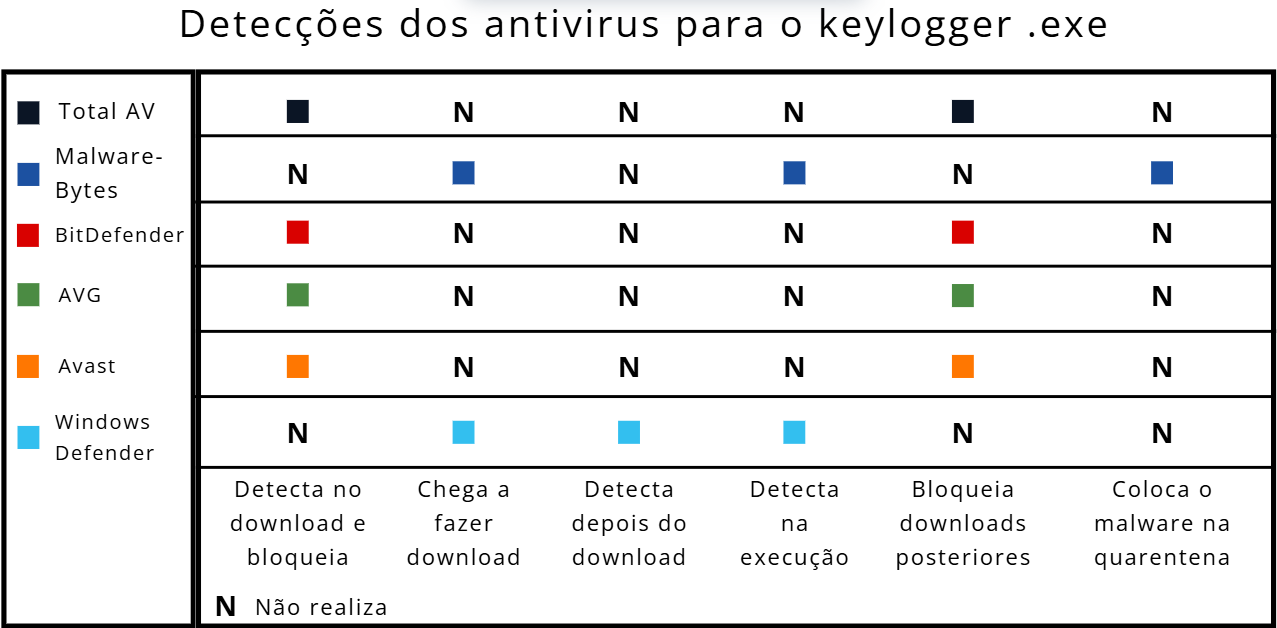
\includegraphics[width=0.8\textwidth]{imgs/exetabelaresultado.png} 
    \caption{Gráfico de resultados dos testes de \textit{keylogger} .exe em máquina.}
\end{figure}

\begin{figure}[H]
    \centering
    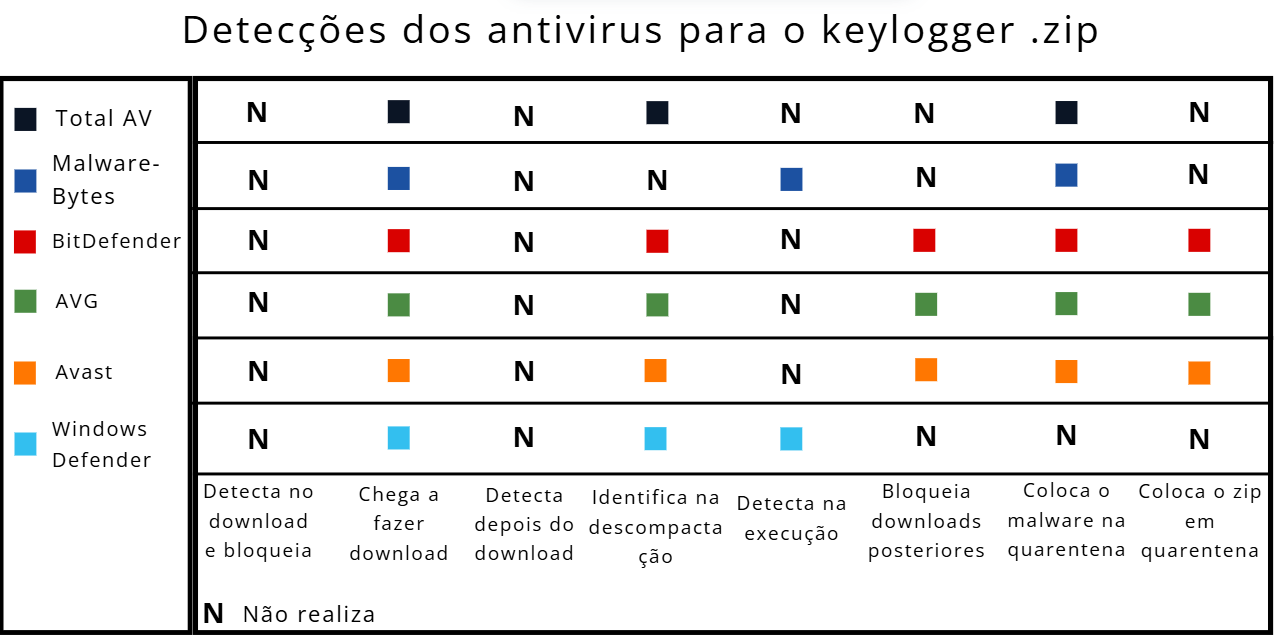
\includegraphics[width=0.8\textwidth]{imgs/ziptabelaresultado.png} 
    \caption{Gráfico de resultados dos testes de \textit{keylogger} zip em máquina.}
\end{figure}

\begin{figure}[H]
    \centering
    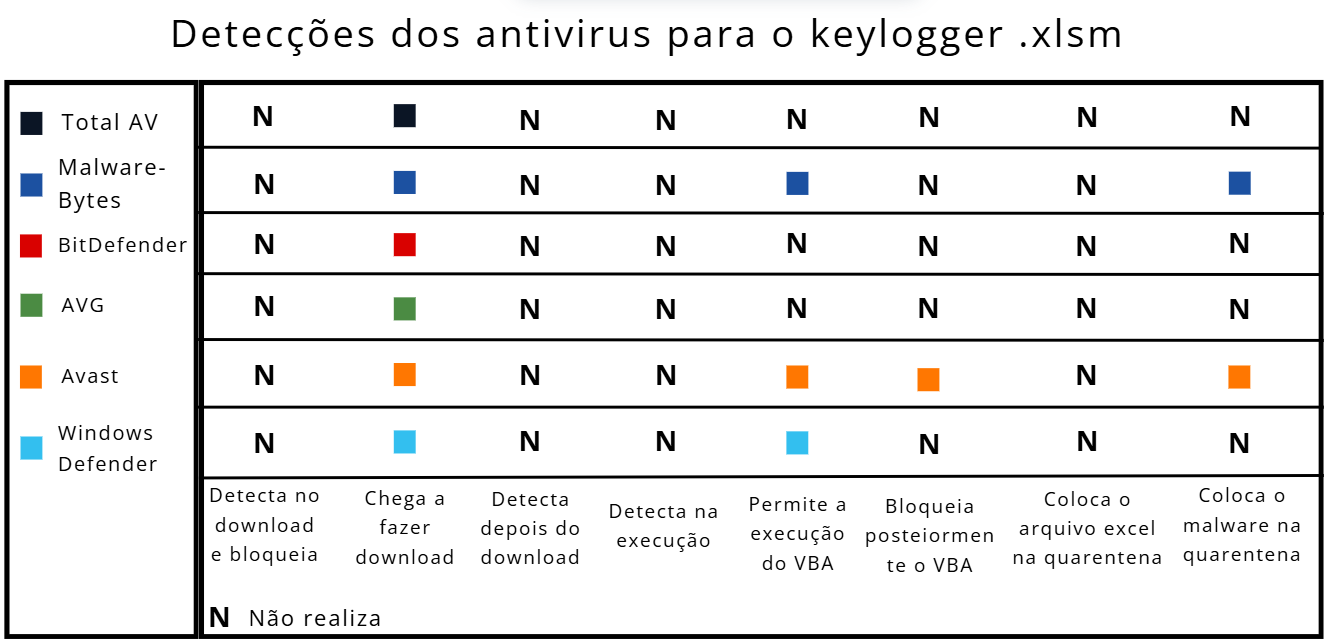
\includegraphics[width=0.9\textwidth]{imgs/xlsmtabelaresultado.png} 
    \caption{Gráfico de resultados dos testes de \textit{keylogger} xlsm em máquina.}
\end{figure}



\subsection*{Detalhes dos resultados}
Windows Defender:
\begin{itemize}
    \item \textbf{Arquivo \texttt{.exe}}: A detecção é inconsistente. Em 40\% dos casos, o arquivo malicioso é detectado, enquanto nos outros não. No entanto, em todos os casos, a execução é bloqueada com um aviso de programa malicioso.
    \item \textbf{Arquivo \texttt{.zip}}: Não detecta o conteúdo malicioso dentro do arquivo compactado. Após a extração, a detecção é inconsistente com cerca de 60\% dos casos posivos, mas sempre bloqueia a execução com um aviso de programa malicioso.
    \item \textbf{Arquivo \texttt{.xlsm}}: Não identifica o download do arquivo malicioso feito via código VBA no \texttt{.xlsm}, permitindo sua execução sem bloqueios.
\end{itemize}

\noindent Avast:
\begin{itemize}
    \item \textbf{Arquivo \texttt{.exe}}: Detecta e bloqueia o arquivo malicioso imediatamente, impedindo o download ainda durante o processo de download do arquivo temporário. Também bloqueia posteriormente o download do arquivo \texttt{.exe} na fonte original.
    \item \textbf{Arquivo \texttt{.zip}}: Após a extração, o arquivo malicioso é detectado e colocado em quarentena, e o próprio arquivo \texttt{.zip} é colocado em quarentena após uma segunda tentativa de extração. O Avast posteriormente também bloqueia o download do \texttt{.zip} na fonte.
    \item \textbf{Arquivo \texttt{.xlsm}}:  Detecta o arquivo .exe após a execução de download do VBA e desativa futuras execuções do Macro no arquivo xlsm. Consequentimente o \textit{keylogger} não é executato.
    \item \textbf{Acesso}: Remove o acesso remoto.
\end{itemize}

\noindent AVG:
\begin{itemize}
    \item \textbf{Arquivo \texttt{.exe}}: Detecta e bloqueia o arquivo malicioso imediatamente, impedindo o download durante o processo de download do arquivo temporário. Também bloqueia o download do arquivo \texttt{.exe} na fonte original.
    \item \textbf{Arquivo \texttt{.zip}}: Após a extração, o arquivo malicioso é detectado e colocado em quarentena, e o próprio arquivo \texttt{.zip} também é colocado em quarentena após uma segunda tentativa de extração. O AVG posteriormente também bloqueia o download do \texttt{.zip} na fonte.
    \item \textbf{Arquivo \texttt{.xlsm}}: Bloqueia o acesso do código VBA aos diretórios da máquina, impedindo o download e a execução do código.
    \item \textbf{Acesso}: Remove o acesso remoto.
\end{itemize}

\noindent Bitdefender:
\begin{itemize}
    \item \textbf{Arquivo \texttt{.exe}}: Detecta e bloqueia o arquivo malicioso imediatamente, impedindo o download durante o processo de download do arquivo temporário. Também bloqueia o download do arquivo \texttt{.exe} na fonte original.
    \item \textbf{Arquivo \texttt{.zip}}: Após a extração, o arquivo malicioso é detectado e bloqueado, mas de maneira lenta, permitindo sua execução momentânea antes do bloqueio.
    \item \textbf{Arquivo \texttt{.xlsm}}: Bloqueia o acesso do código VBA aos diretórios da máquina, impedindo o download e a execução do código.
    \item \textbf{Acesso}: Remove o acesso remoto.
\end{itemize}

\noindent{MalwareBytes}
\begin{itemize}
    \item \textbf{Arquivo \texttt{.exe}}: Não detecta o arquivo durante o download, mas bloqueia sua execução quando o identifica como \textit{malware}, colocando-o em quarentena.
    \item \textbf{Arquivo \texttt{.zip}}: Não detecta o conteúdo malicioso dentro do arquivo compactado durante o download ou na extração. Apenas bloqueia o arquivo \texttt{.exe} ao ser executado, colocando-o em quarentena.
    \item \textbf{Arquivo \texttt{.xlsm}}: A detecção e o bloqueio ocorrem apenas durante a execução do \texttt{.exe}. O download do \texttt{.exe} é permitido, mas sua execução é bloqueada. (Apenas na execução o arquvo é detectado) \textit{Keylogger} não é executato.
\end{itemize}

\noindent Total AV:
\begin{itemize}
    \item \textbf{Arquivo \texttt{.exe}}: Detecta e bloqueia o arquivo malicioso imediatamente, impedindo o download durante o processo de download do arquivo temporário. Também bloqueia o download do arquivo \texttt{.exe} na fonte original.
    \item \textbf{Arquivo \texttt{.zip}}: Não detecta o conteúdo malicioso durante o download. Após a extração, o arquivo malicioso é detectado e bloqueado. Não exclui o .zip e nem bloqueia seu downloand na fonte.
    \item \textbf{Arquivo \texttt{.xlsm}}: Bloqueia o acesso do código VBA aos diretórios da máquina, impedindo o download e a execução do código.
\end{itemize}

\noindent Nenhum dos programas antivirus testados detecta o arquivo \texttt{.xlsm} como malicioso, nem o conteúdo do arquivo \texttt{.zip} durante o primeiro momento de download.

\section{Conclusão e trabalhos futuros}
Com base nos resultados obtidos neste trabalho, 
é possível concluir que os diferentes motores de antivirus 
apresentam níveis variados de eficácia na detecção de um \textit{keylogger}, 
dependendo do formato do arquivo e das técnicas empregadas para sua ocultação. 
Os testes realizados com os métodos de infecção em formato .exe, .zip e .xlsm demonstraram que, 
quanto mais complexas são as técnicas de infecção, como ofuscação de código e uso de macros 
em documentos legítimos, maior é a dificuldade dos sistemas de segurança em identificá-las.

Os seguintes antivirus se destacaram e podem ser indicados conforme o cenário analisado:  
\textbf{.exe}: Todos os quatro antivirus testados (\textbf{Avast}, \textbf{AVG}, \textbf{Total AV} e \textbf{Bitdefender}) foram eficazes em detectar e bloquear o \textit{keylogger}, sendo capazes de impedir seu funcionamento logo durante o download.  
\textbf{.zip}: O \textbf{Avast} e o \textbf{AVG} mostraram-se mais eficientes na identificação do conteúdo malicioso, especialmente após a extração do arquivo compactado.  
\textbf{.xlsm}: O \textbf{Bitdefender}, o \textbf{AVG} e o \textbf{Total AV} destacaram-se, pois conseguiram bloquear o acesso do código VBA aos diretórios da máquina, mesmo que nenhum tenha identificado o conteúdo malicioso de maneira totalmente proativa.

Em trabalhos futuros, a aplicação da técnica de engenharia reversa a \textit{keyloggers} pode 
proporcionar uma compreensão mais aprofundada de suas estruturas internas e métodos de evasão, 
o que contribuiria para o desenvolvimento de assinaturas e padrões de detecção mais eficazes. Além disso, 
testar \textit{keyloggers} utilizando métodos de infecção mais eficientes, 
como contaminação por rede, pode ajudar a fortalecer ainda mais o cenário da segurança digital.


\bibliographystyle{plainnat}
\bibliography{sbc-template.bib}
\end{document}
